\documentclass[a4paper]{article}
\usepackage{ucs}  % unicode
\usepackage[utf8x]{inputenc}
% \usepackage[T2A]{fontenc}
% \usepackage[bulgarian]{babel}
\usepackage{graphicx}
% \usepackage{fancyhdr}
% \usepackage{lastpage}
\usepackage{listings}
\usepackage{slashbox}
\usepackage{multirow}
\usepackage{wrapfig}
% \usepackage{fancyvrb}
% \usepackage[usenames,dvipsnames]{color}
% \setlength{\headheight}{12.51453pt}

%\pagestyle{fancy}
%\fancyhead{}
%\fancyfoot{}

% \cfoot{\thepage\ от \pageref{LastPage}}

% \addto\captionsbulgarian{%
%   \def\abstractname{%
%     Цел на проекта} %\cyr\CYRA\cyrs\cyrt\cyrr\cyra\cyrk\cyrt}}%
% }

% Custom defines:
\def\definition{Definition:\ }
\def\la{\leftarrow}
\def\vars{\mathrm{Vars}}
\def\occ{\mathrm{Occ}}
% \def\dc{bar baz}

% TODO remove colorlinks before printing
% \usepackage[unicode,colorlinks]{hyperref}   % this has to be the _last_ command in the preambule, or else - no work
% \hypersetup{urlcolor=blue}
% \hypersetup{citecolor=PineGreen}

\begin{document}

\newcommand{\aee}[1] {[[#1]]^\sharp}
\newcommand{\cc}[1] {\texttt{#1}}
\def\A {\mathcal{A}}
\def\N {\mathcal{N}}
\def\NonZero {\mathrm{NonZero}}
\def\Zero {\mathrm{Zero}}
\def\Vars {\mathrm{Vars}}
\def\Occ {\mathrm{Occ}}

\title{Static Program Analysis - Exercise 3}
\author{Iskren Ivov Chernev \\ tutorial group B}

\maketitle

\section{Solution}

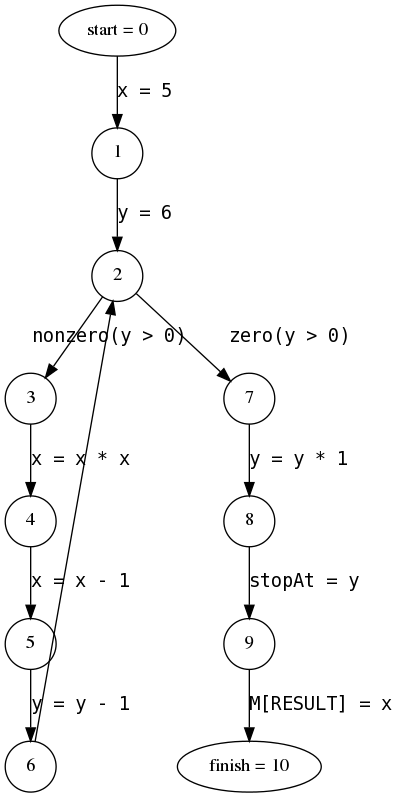
\includegraphics[scale=0.3]{3-1.png}
% \begin{wrapfigure}{r}{0cm}
%   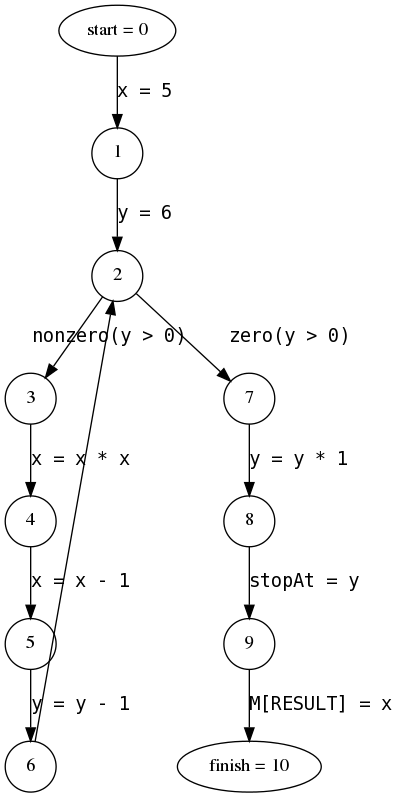
\includegraphics[scale=0.3]{3-1.png}
% \end{wrapfigure}
\begin{tabular}{|c|c|c|}
  \hline
  \multicolumn{3}{|c|}{Live variables} \\
  \hline
            & 1   &  2  \\ \hline
  $ A[10] $ & $ \emptyset $           & \multirow{10}{*}{dito} \\ \cline{1-2}
  $ A[9] $  & $ \{ x, RESULT \} $     & \\ \cline{1-2}
  $ A[8] $  & $ \{ x, y, RESULT \} $  & \\ \cline{1-2}
  $ A[7] $  & $ \{ x, y, RESULT \} $  & \\ \cline{1-2}
  $ A[2] $  & $ \{ x, y, RESULT \} $  & \\ \cline{1-2}
  $ A[6] $  & $ \{ x, y, RESULT \} $  & \\ \cline{1-2}
  $ A[5] $  & $ \{ x, y, RESULT \} $  & \\ \cline{1-2}
  $ A[4] $  & $ \{ x, y, RESULT \} $  & \\ \cline{1-2}
  $ A[3] $  & $ \{ x, y, RESULT \} $  & \\ \cline{1-2}
  $ A[1] $  & $ \{ x, RESULT \} $     & \\ \cline{1-2}
  $ A[0] $  & $ \{ RESULT \} $        & \\ \hline
\end{tabular}

\vspace{1cm}

\begin{tabular}{|c|c|c|}
  \hline
  \multicolumn{3}{|c|}{Truly live variables} \\
  \hline
            & 1   &  2  \\ \hline
  $ A[10] $ & $ \emptyset $           & \multirow{10}{*}{dito} \\ \cline{1-2}
  $ A[9] $  & $ \{ x, RESULT \} $     & \\ \cline{1-2}
  $ A[8] $  & $ \{ x, RESULT \} $     & \\ \cline{1-2}
  $ A[7] $  & $ \{ x, RESULT \} $     & \\ \cline{1-2}
  $ A[2] $  & $ \{ x, y, RESULT \} $     & \\ \cline{1-2}
  $ A[6] $  & $ \{ x, y, RESULT \} $     & \\ \cline{1-2}
  $ A[5] $  & $ \{ x, y, RESULT \} $     & \\ \cline{1-2}
  $ A[4] $  & $ \{ x, y, RESULT \} $     & \\ \cline{1-2}
  $ A[3] $  & $ \{ x, y, RESULT \} $     & \\ \cline{1-2}
  $ A[1] $  & $ \{ x, RESULT \} $     & \\ \cline{1-2}
  $ A[0] $  & $ \{ RESULT \} $        & \\ \hline
\end{tabular}

\section{Solution}
\begin{verbatim}
/* heavily influenced by the Live_Variables example analysis */
TYPE

  VarSetLifted = lift(VarSet)


PROBLEM Truly_Live_Variables

  direction  : backward
  carrier    : VarSetLifted
  init       : bot
  init_start : lift({})
  combine    : lub


TRANSFER

  ASSIGN(variable, expression) =
      let lifeVars <= @ in
        lift((lifeVars - variable) lub if     variable ? lifeVars
                                       then   variables(expression)
                                       else   {}  /* here is the only change */
                                       endif)

  IF(expression) =
      let lifeVars <= @ in
        lift(lifeVars lub variables(expression))
  
  WHILE(expression) =
      let lifeVars <= @ in
        lift(lifeVars lub variables(expression))

  CALL(_, _, expression) =
      let lifeVars <= @ in
        lift(lifeVars lub variables(expression))

  RET(_, param, _), local_edge =
      let lifeVars <= @ in
        lift({x | x in lifeVars; x = param })

  BEGIN(_, param), call_edge =
      let lifeVars <= @ in
        lift({x | x in lifeVars; x != param })


SUPPORT

  subExpressions :: Expression -> ExpressionSet
  subExpressions(expression) =
    case expType(expression) of
      "ARITH_BINARY" => subExpressions(expSubLeft(expression)) lub
                        subExpressions(expSubRight(expression));
      "ARITH_UNARY"  => subExpressions(expSub(expression));
      "BOOL_BINARY"  => subExpressions(expSubLeft(expression)) lub
                        subExpressions(expSubRight(expression));
      "BOOL_UNARY"   => subExpressions(expSub(expression));
      _              => {}; 
    endcase
    + expression

  variables :: Expression -> VarSet
  variables(expression) =
    { expVar(exp) | exp in subExpressions(expression);
                    expType(exp) = "VAR" }
\end{verbatim}

\section{Solution}
  For dead variables (as opposed to live variables):
  \begin{itemize}
    \item nop $ [[;]]^\sharp D = D $
    \item condition $ [[\NonZero(e)]]^\sharp D = [[\Zero(e)]]^\sharp D = D \setminus \Vars(e) $
    \item load $ [[x \la e]]^\sharp D = [[x \la M[e]\;]]^\sharp D = (D \cup \{ x \}) \setminus \Vars(e) $
    \item store $ [[M[e_1] \la e_2]]^\sharp = D \setminus \{ \Vars(e_1) \cup \Vars(e_2) \} $
  \end{itemize}

  For truly dead variables (as opposed to truly live variables) only change load edge effects:
  \begin{itemize}
  \item load $ [[x \la e]]^\sharp D = [[x \la M[e]\;]]^\sharp D = (D \cup \{ x \}) \setminus (x \in D\ ?\ \emptyset : \Vars(e)) $
  \end{itemize}

  Path ($ \pi = k_1 k_2 \dots k_n $) effect is formed by combining the edge
  effects along it (in reverse order, since it is a backward analysis):
  $$
    \aee{\pi} = \aee{k_1} \circ \aee{k_2} \circ \dots \circ \aee{k_n}
  $$

  To obtain the dead variable information at a particular program point we
  intersect the dead variables from all possible paths from that point to the
  program end. We use intersect, because if a variable is not dead along one
  path, than it is not dead at the point. Initially (i.e. at the end of the
  program) all variables are considered dead.
  $$
    \mathcal{D}^\star[v] = \bigcup \{\ \aee{\pi} \Vars\ |\ \pi = v \longrightarrow^\star \mbox{end}\ \}
  $$
  
\section{Solution}

Variables, that are first read are found by the live/dead variable analysis
that we studied. We only need the result of the analysis at the beginning of
a program, because parameters only make sense at program start. If we consider
a variable to be a parameter, if on all paths it is first read, then we should
change the live variable MOP formula from set union to set intersection, i.e.
to obtain ``everywhere live'' variables -- variables that are live on all paths
of execution. Either ``live variables'' or ``truly live variables'' will
suffice as a base analysis.

\section{Solution -- todo}

\end{document}
